% !TEX root = document.tex

\lstdefinestyle{mystyle_ex_stratego_program}{
language = Python,
morekeywords = {1, 2, r1, r2, Exp, E, Null, A, B, prog, Plus},
keywordstyle = [2]{\color{num_color}},
morekeywords = [2]{1, 2},
keywordstyle = [3]{\color{kw_alt}},
morekeywords = [3]{signature, sorts, constructors, Int, strategies, topdown, rules, add}
}
\lstdefinestyle{mystyle_automaton_pseudo}{
language = Python,
morekeywords = {Map, put, contains, get},
keywordstyle = \color{kw_alt},
keywordstyle = [2]{\color{magenta}},
morekeywords = [2]{Statement, Constructor, Automaton, automatonMap, constructAutomata, build, buildStatementAutomaton, getChild, addToStart, addTransition}
}
\lstdefinestyle{mystyle_fused_stratego}{
language = Python,
morekeywords = {r1, r2, Null, A, B, f_main, f_main_A, f_main_B, f_main_Null, f_0, f_0_A, f_0_B, f_0_Null, f_1, f_1_A, f_1_B, f_1_Null},
keywordstyle = [2]{\color{kw_alt}},
morekeywords = [2]{id}
}

\chapter{\label{chap:solution}A Traversal Fusion Algorithm for Strategic Programming}

In this chapter, we describe the algorithm that we have developed for generic traversal fusion in strategic programming. This algorithm predicts opportunities for traversal fusion by performing a dependency analysis on the program as a whole (i.e. its traversals and rewrite rules).

By analyzing the operations that rewrite rules perform, as well as how the traversals interact with this process, it is possible to construct a (partial) order that specifies which operations need to happen before others in the program. The algorithm then attempts to fuse together the recursive call operations that make up the traversals of the program. In case any two such statements can be fused without causing a dependency cycle, traversal fusion can be performed on those calls.

The algorithm consists of five main steps based on both the TreeFuser and Grafter algorithms \cite{SakkaS017, SakkaSN019}, each of which will be described in detail in the following. The steps are:
\begin{enumerate}
    \item Parsing and extracting the necessary information from the source program;
    \item Performing a dependency analysis on the rewrite rules and traversals;
    \item Building a dependence graph from the dependency analysis results;
    \item Finding fusion opportunities in the dependence graph;
    \item Synthesizing a program with fused traversals.
\end{enumerate}

\section{Soundness of Fusion with Dependency Analysis}
Before exploring the algorithm in more detail, we will touch on why the approach that predicts fusion opportunities using dependency analysis is sound. A thorough analysis of the soundness of this approach has been done, which identified two criteria that a sound fusion must satisfy: preservation of work and preservation of dependencies \cite{SakkaS017, SakkaSN019}. In short, the fused version of a program must perform exactly those operations on nodes that were performed in the original program, and if two operations have a dependency relation, they must be performed in the same order as in the original program.

Note that these criteria are true in general, regardless of the approach taken to fusion. The intuition here is that, if two operations on a node do not have a dependency relation, it cannot possibly matter for the final result in which order these operations are performed. Then, any program that performs the exact same operations while respecting all dependency relations must lead to the same result.

This, of course, logically leads to using dependency analysis to predict fusion opportunities, as it directly satisfies the dependency relation criterion. The other criterion is relatively easily satisfied by not touching the rewrite rules in our case.

\section{Information Extraction}
The most important pieces of information required from the source program are the outline of the program (i.e. which traversals are used and in which order), the definitions of the rewrite rules used in those traversals, as well as information about the constructors and their types.

In Stratego, this information is extracted using the standard parser for the language. The prototype implementation only supports a subset of the Stratego language and makes some assumptions about the format of the input program.

Specifically, we require:
\begin{itemize}
    \item A declaration of all sorts, and all constructors and their types
    \item Constructors to only be simple types using the declared sorts (e.g. no list types)
    \item A single main strategy called \texttt{prog} that consists of a sequence of calls to \texttt{all}, rule applications, calls to the built-in strategies \texttt{topdown} or \texttt{bottomup}, or calls to other strategies using only these features
    \item Rewrite rules to only perform pure rewrites without side effects (function calls are allowed)
\end{itemize}

These limitations will be discussed in more detail in \autoref{sec:limitations}, including an analysis of which limitations are inherent to the algorithm, and which limitations exist only due to time constraints, including suggestions on how to address them.

After extracting the necessary information, some processing is required before we continue to the next step. Note that what appears to be a single rewrite rule is actually a set of rewrite rules with the same label in Stratego, and a single label can consequently have an arbitrary number of definitions. The left-hand side of such a definition is a match statement (which could and usually does match on the constructor). This means the constructor changes which rewrite rules within a rewrite rule set are active. This has significant implications for the dependency analysis, because a ruleset could do something completely different on a different constructor. As such, each ruleset is separated into multiple virtual sets differentiated by the constructor in their left-hand side match statement for the dependency analysis.

An example of a program that can be analyzed using this algorithm has been included in \autoref{fig:ex-stratego-program}, and will also be used as an example throughout this chapter. This program does not compute anything useful, but serves as a good illustration of the possible different cases that can occur while executing the algorithm.

\begin{figure}
\begin{lstlisting}[style = mystyle_ex_stratego_program]
    signature
      sorts
        Exp

      constructors
        Null : Exp
        A : Exp * Exp * Int * Int -> Exp
        B : Exp * Int -> Exp

    strategies
      prog = topdown(r1); topdown(r2)

    rules
      r1 :
        Null() -> Null()
    
      r1 :
        A(l, r, a, b) -> A(l, r, (<add> (a, b)), b)

      r1 :
        B(c, v) -> B(c, (<add> (v, 1)))

      r2 :
        Null() -> Null()

      r2 :
        A(A(ll, lr, la, lb), r, a, b) -> A(A(ll, lr, la, lb), r, (<add> (a, la)), b)

      r2 :
        A(B(c, v), r, a, b) -> A(B(c, v), r, (<add> (a, v)), b)

      r2 :
        B(c, v) -> B(c, (<add> (v, 1)))
\end{lstlisting}

\caption{Example Stratego program to be analyzed.}
\label{fig:ex-stratego-program}
\end{figure}

\section{Dependency Analysis}
The dependency analysis determines the \textit{reads} and \textit{writes} made by all the rewrite rules. These terms refer to locations that are read from or written to by a rewrite rule, respectively. We give an exact definition in the context of strategic programming later on in this chapter.

After analyzing the rewrite rules, the dependency analysis determines the reads and writes of the recursive calls of a traversal. This is a necessary step in building the (partial) execution order of the program.

\subsection{Access Paths and Access Automata}
The dependency analysis makes use of access paths and access automata.

Access paths are a generic way of discussing locations relative to a certain node. The children of a node are numbered from left to right, starting from 0. Then, for example, the left child of a node with two children can be referred to with \texttt{n.0}, and its right child with \texttt{n.1} (with \texttt{n} always referring to the current node). Access paths are, in essence, regular expressions. Further descendants can thus easily be pointed to with \texttt{n.0.0}, \texttt{n.0.1}, and so on. Furthermore, \texttt{n(.0)*} could point to \texttt{n}, \texttt{n.0}, \texttt{n.0.0}, etc. When constructing the reads and writes of traversals, these paths will become more complex, and it is easier to construct them as their equivalent automata. These are called access automata.

\subsection{Type-Specific Analysis}
In the dependency analysis, the algorithm cannot make any assumptions about the structure of the input data other than the information gathered from the constructor definitions. And because strategies are generic, it is not possible to know the type of the node they will be called on, the types of its children, or even its number of children. In addition, note again that rewrite rules are actually sets that may have multiple definitions (differentiated by the constructor of the node they are executed on). Consequently, the dependency analysis has to be performed separately for every possible constructor.

The logical conclusion of the previous statement is that it may be possible to fuse certain strategies when executing on one constructor, but not on another. This is the type-specific partial fusion discussed in \autoref{sec:towards-a-solution}.

Note that this type-specific analysis, in most cases, makes the analysis more complex than simpler. Consider the \texttt{A} and \texttt{B} constructors in \autoref{fig:ex-stratego-program}. They both are constructors of the \texttt{Exp} sort, and also each have children of the \texttt{Exp} sort. This means they are mutually recursive and their dependency analyses, while performed separately, may still need to interact with each other.

\subsection{Rewrite rules}
Determining the reads and writes of the rewrite rules is required to determine the reads and writes of the traversals. Rewrite rules in strategic languages do not read and write to locations in the same way as might occur in an imperative language. The notions of reading and writing will be defined as follows:

A rewrite rule has a left-hand side, and a right-hand side. On the left, it performs a match to determine whether the rule applies to the current node. This can be considered to be a read, because the necessary terms need to be read to determine whether the match applies to this node. A match statement does not necessarily always read all the children of a node. For example, consider the following rule:

\begin{lstlisting}[style = mystyle_ex_stratego_program]
    Plus(left, right) -> Plus(left, 1)
\end{lstlisting}

Despite both \texttt{left} and \texttt{right} being named in this rule, neither is ever read. Nothing happens to \texttt{left}, and \texttt{right} is always overwritten, regardless of what its value was.

In contrast, a rule such as
\begin{lstlisting}[style = mystyle_ex_stratego_program]
    Plus(left, 1) -> Plus(left, 2)
\end{lstlisting}

Does perform a read on the child that was called \texttt{right} in the previous rule (i.e. the location \texttt{n.1}). It has to be read to check whether its value is \texttt{1}, in order to determine whether the rewrite rule applies.

Then, if a location is not assigned a variable, but instead is matched on with a concrete value, it is \textit{always} read. If a location \textit{is} assigned a variable, it may or may not be read. Consider this rule:
\begin{lstlisting}[style = mystyle_ex_stratego_program]
    Plus(left, right) -> Plus(right, right)
\end{lstlisting}

Here, the location \texttt{n.1} \textbf{is} read, because its value has to be copied to \texttt{n.0}. The notion of reading in the context of a dependency analysis does include copying: while it is theoretically possible to copy a value in memory without reading its contents, this still introduces a read dependency. That is to say, if a later statement were to alter the value in \texttt{n.1}, it would \textbf{not} be legal to move that statement before this one in the program.

From this, the following concrete rules are derived to determine whether a location is read:
\begin{enumerate}
    \item If a location \textbf{is matched on with a concrete value}, it is always read.
    \item Otherwise, if a location is assigned a variable, it is read \textbf{only} if that variable occurs in a different location on the right-hand side.
\end{enumerate}

Writes are simpler to analyze: a location is written to if and only if its value on the right-hand side is not equal to its value on the left-hand side.

Finally, the algorithm also supports wildcards and calls to pure functions in rewrite rules.

Wildcards can only occur on the left-hand side. Locations matched with a wildcard are never read, but always written to.

Function calls can only occur on the right-hand side. They always write to their location. Their reads are a union of all their function arguments. It is legal to ignore what the function actually does internally because it is pure: for the purposes of the dependency analysis, calling a function is identical to writing a tuple of all the function arguments to a location.

\subsection{Correctly Constructing Automata}
The rules in the previous section define what reads and writes are in the context of rewrite rules. However, some additional rules are necessary to correctly construct access automata for the dependency analysis.

First, in the case of a rewrite ruleset with multiple definitions, the reads and writes of all definitions that apply to the constructor currently being analyzed can be combined. We use an automaton union algorithm for this.

Second, and most importantly, all prefixes of the read and write automata constructed also need to be considered:

\begin{itemize}
    \item For read automata, every prefix is also read. That means that every state except the initial state is an accept state.
    \item For write automata, only the final state is an accept state. However, all prefixes are read, and as such should be added to the rewrite rule's read automaton.
\end{itemize}

Equivalently, we could say that both read and write automata always read all their prefixes. The intuitive reason for this is that these prefixes represent the parent nodes of the location being referenced with the automaton, and writing to one of the parents should cause a dependency conflict with the child as well.

It is perhaps better illustrated with an example: two rewrite rules operating on a binary tree as seen below.

\begin{lstlisting}[style = mystyle_ex_stratego_program]
    r1: E(E(ll, lr), r) -> E(E(ll + 1, lr), r)
    r2: E(_, r) -> E(r, r)
\end{lstlisting}

The first reads and writes to location \texttt{n.0.0}, while the second writes to \texttt{n.0}. Without considering prefixes, these two rewrite rules would not conflict, and the second could theoretically be moved in front of the first. However, that should be illegal: the write to \texttt{n.0} implicitly overwrites the value in \texttt{n.0.0}. In the original execution order, that would be the final value stored in the node. If the rewrite rules were swapped, that value would be incremented by one.

\subsection{Traversals}
With the reads and writes of the rewrite rules determined, it becomes possible to define the reads and writes of the traversals. The core idea is to analyze traversals as recursive functions, consisting of statements that apply rewrite rules, and calls that call a function on one or multiple child nodes. We are now interested in determining the reads and writes of these calls.

The reads and writes for calls must be analyzed in a type-partial way. So, the algorithm considers every constructor and analyzes the reads and writes of a call, given that it is executed on a node of that constructor. The \texttt{all} function (that executes it argument on every child of a node) is split into multiple individual calls for every child (which is now possible because we know how many children this constructor has).

The actual reads and writes of such a call, then, are defined recursively. Consider, for example, \texttt{r1} from the example given in \autoref{fig:ex-stratego-program}, executing on a node with constructor \texttt{B}. This rule both reads and writes to the location \texttt{n.1}. Ignoring the possibility of a child with constructor \texttt{A} for now, executing this rule \texttt{topdown} would cause it to be applied recursively on the left child. This means the call to the left child reads and writes \texttt{n.0.1}, \texttt{n.0.0.1}, etc. This is precisely what is needed for the dependency analysis.

If we do consider the possibility for a child with constructor \texttt{A}, these access paths quickly become more complex. The algorithm therefore is based on constructing access automata. 

\autoref{fig:traversal-dependency-pseudocode} shows the pseudocode of the algorithm that constructs the dependency automata.

This algorithm recursively constructs a set of automata representing the read and write dependencies for every statement in the program executing on every possible constructor. These automata are mutually recursive, but the algorithm is guaranteed to terminate because if an automaton has already been constructed for a certain statement executing on a certain constructor, a reference to that automaton is simply inserted instead of creating a new one.

\subsection{Example Construction}
To illustrate the read/write analysis and the construction of the read/write automata more clearly, we will use the example program from \autoref{fig:ex-stratego-program}. The automata will be built up step by step in \autoref{fig:ex-automata}. We will build the automata per constructor, starting with \texttt{Null}.

\texttt{Null} has no children, which means it does not perform calls. There are only two statements to analyze: the one representing the application of \texttt{r1}, and the one representing the application of \texttt{r2}. Neither \texttt{r1} nor \texttt{r2} perform reads or writes on \texttt{Null}. As such, both statements generate an automaton with a single non-accepting start state with no edges (equivalent to an empty automaton).

Next, we look at the constructor \texttt{B}. It does have a single child on which a traversal can be called, and the rewrite rules do perform an operation on nodes with this constructor. This means there are four statements in total to analyze: one for each rewrite rule application, one call statement (on the only child) from the first traversal, and one call from the second traversal. We label the first call \texttt{c0}, and the second \texttt{c1}. First, we note that \texttt{r1} and \texttt{r2} are equivalent for \texttt{B}. They perform a single read and write, on \texttt{n.1}. We have now arrived at the situation seen in \autoref{fig:r_w_2}. Next, we will look at the call statements. There are two functions that can be called, corresponding to the two traversals. These functions consist of the rewrite rule application statements, as well as the traversal call statements. \texttt{B}'s child is of type \texttt{Exp}, which means its constructor can be either \texttt{A}, \texttt{B}, or \texttt{Null}.

We start with a single non-accepting start state for each call statement. In case the child constructor is \texttt{Null} or \texttt{B}, the following happens: the algorithm sees that the automata for all statements in the called function on that constructor have already been generated (the automaton for the call on \texttt{B} is a reference to the one currently being constructed). \texttt{B}'s child lives at index \texttt{0}, and as such edges labeled with \texttt{0} are added, pointing to all the automata for every statement in the function being called. This is illustrated in \autoref{fig:r_w_3}.

We also have to consider the case in which \texttt{B}'s child has constructor \texttt{A}. This will trigger the dependency analysis for the \texttt{A} constructor. It has more statements because it has two children instead of one: there are still two rewrite rule application statements, but there are now four call statements (one per child per traversal). \texttt{c0} is the call on the left child from the first traversal, \texttt{c1} the call on the right child from the first traversal. \texttt{c2} and \texttt{c3} are the calls on the left and right children respectively from the second traversal. \texttt{r1} on \texttt{A} reads \texttt{n.2} and \texttt{n.3}, and writes to \texttt{n.2}. \texttt{r2} also writes to \texttt{n.2}, but reads \texttt{n.0}, \texttt{n.0.1}, \texttt{n.0.2}, and \texttt{n.2}. This creates the automata seen in \autoref{fig:r_w_4}.

\texttt{A}'s children are also of type \texttt{Exp}, and as such can have constructor \texttt{A}, \texttt{B}, or \texttt{Null}. All other automata have now been constructed, so the insertion of the reference edges proceeds in the same way. Edges from \texttt{B}'s calls pointing to \texttt{A} can now also be inserted. The final construction is seen in \autoref{fig:r_w_5}.

\begin{figure}
\centering
\begin{subfigure}{0.45\textwidth}
\centering
\raisebox{39pt}{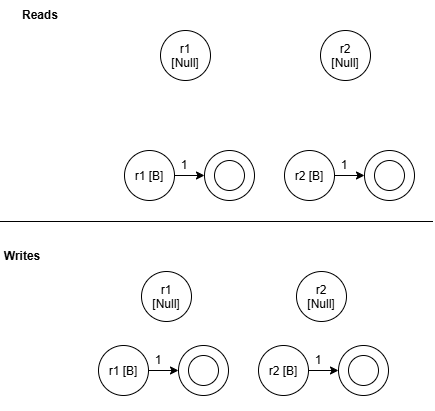
\includegraphics[width=\linewidth]{./img/r_w_2.png}}
\subcaption{Step 1.}
\label{fig:r_w_2}
\end{subfigure}%
\begin{subfigure}{0.45\textwidth}
\centering
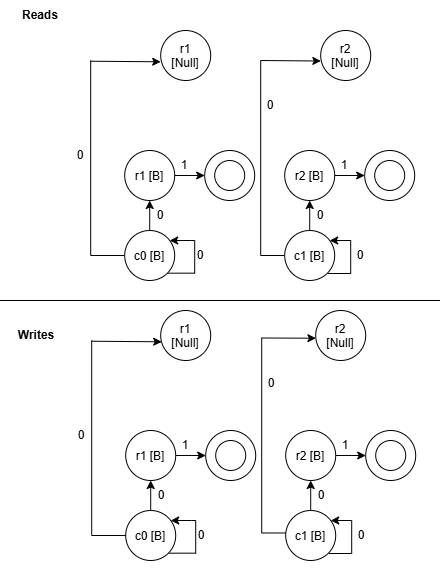
\includegraphics[width=\linewidth]{./img/r_w_3.png}
\subcaption{Step 2.}
\label{fig:r_w_3}
\end{subfigure}

\begin{subfigure}{0.45\textwidth}
\centering
\raisebox{25pt}{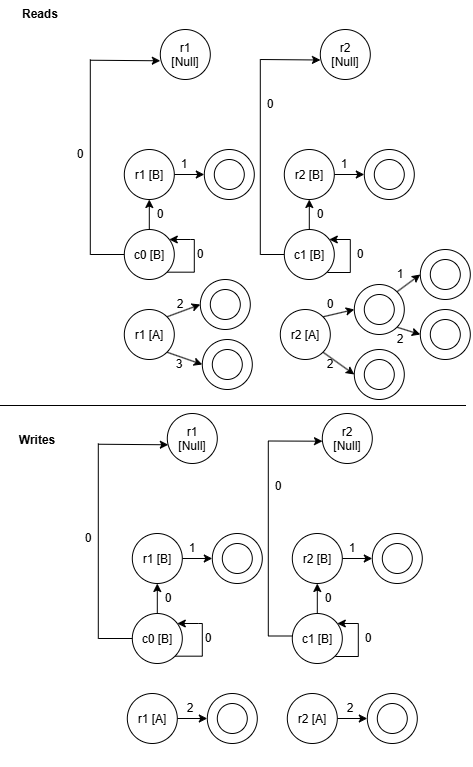
\includegraphics[width=\linewidth]{./img/r_w_4.png}}
\subcaption{Step 3.}
\label{fig:r_w_4}
\end{subfigure}%
\begin{subfigure}{0.45\textwidth}
\centering
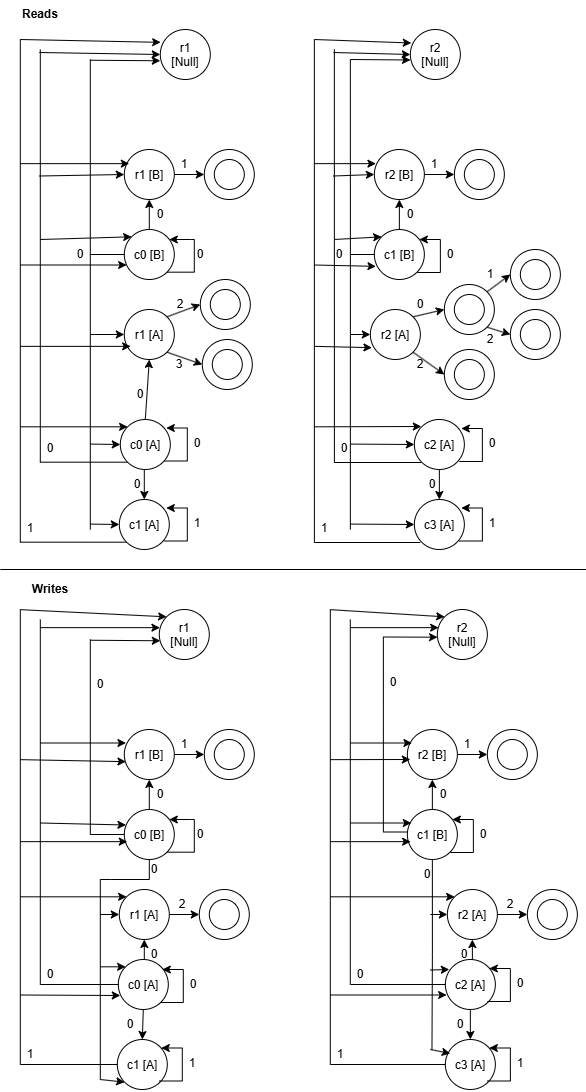
\includegraphics[width=\linewidth]{./img/r_w_5.png}
\subcaption{Step 4.}
\label{fig:r_w_5}
\end{subfigure}

\caption{Read/write automaton construction for the example program in \autoref{fig:ex-stratego-program}.}
\label{fig:ex-automata}
\end{figure}

\begin{figure}
\begin{lstlisting}[style = mystyle_automaton_pseudo]
Map<(Statement, Constructor) -> Automaton> automatonMap;

constructAutomata():
  for c in possible constructors:
    for f in functions:
      build(c, f)

build(c, f):
  for s in f.statements:
    if s is rewrite rule:
      resultAutomaton = buildStatementAutomaton(s, c)
      automatonMap.put((s, c) -> resultAutomaton)
      return resultAutomaton
    else if s is call:
      child = c.getChild(s.idx)
      resultAutomaton = null;
      for childC in child.possibleConstructors:
        automaton = null;
        if automatonMap.contains((s, c)):
          automaton = automatonMap.get((s, c))
        else:
          automaton = build(childC, s.calledFunction)
        resultAutomaton = addToStart(resultAutomaton, s.idx, automaton)
      automatonMap.put((s, c) -> resultAutomaton)
      return resultAutomaton

addToStart(a1, c, a2):
  a1.startState.addTransition(c, a2.startState)
\end{lstlisting}

\caption{Pseudocode of the traversal dependency analysis algorithm.}
\label{fig:traversal-dependency-pseudocode}
\end{figure}
%With the reads and writes of the rewrite rules determined, we can now also define the reads and writes of the traversals. Essentially, the idea is that analyzing these traversals as recursive functions constructs an access path that is a regular expression. For example, consider the following example of a binary tree and a simple traversal rule that increments a stored value inside a node.%

%\begin{lstlisting}
%    rule:
%      E(left, right, val) -> E(left, right, Plus(val, 1))
%\end{lstlisting}

%We analyze the reads and writes of the rewrite rule using the method described in the previous section. Clearly the only write is to the location \texttt{n.2}, as that is the only location that is changed by the rewrite rule. The only read is also on \texttt{n.2} - note that the variable \texttt{val} does indeed appear in a different location on the right-hand side of the rule (\texttt{n.2.0} instead of \texttt{n.2}).%

%Then, if we were to perform a topdown traversal with this rule, consider what would happen. We execute the rule on the current node (reading and writing to \texttt{n.2}), then go into either the left or right child (\texttt{n.0} or \texttt{n.1}), then execute the rule on those children, and continue into their children, etc.%

%This means the reads and writes performed by the traversal look like this: \texttt{n.2}, \texttt{n.0.2}, \texttt{n.1.2}, \texttt{n.0.0.2}, \texttt{n.0.1.2}, ...%

%Or, in a regular expression, \texttt{n(.0|.1)*.2}%

%Now, we consider the application of the rule to the current node to not be part of the recursive calls for the traversal, and analyze the traversal down into each of the children separately. This means that, in this example of a binary tree, a topdown traversal generates two calls with reads and writes of \texttt{n.0(.0|.1)*.2} and \texttt{n.1(.0|.1)*.2}.%

\section{Building the Dependence Graph}
After performing the dependency analysis, the rules and traversals are analyzed in program order. The notion of program order is not very strictly defined in a strategic language. Whereas one can simply read a program in order in an imperative language, rewrite rules and traversals can be more abstractly defined. In order to overcome this problem, we analyze rewrite rules as single statements that perform all their read and write operations at the same time. This means our fusion algorithm will never pull rewrite rules apart. It is theoretically possible that splitting a rewrite rule into multiple statements could increase fusion opportunities, simply by being more permissive in the program order, but this would also further complicate the algorithm. For traversals, the program order is defined simply as all the recursive calls executed in order. For \texttt{all}, we assume the calls to the children are made left-to-right.

%As mentioned before, the traversals have to be analyzed as recursive functions. For \texttt{topdown}, it is relatively easy to extract a program order from its concrete definition. It executes the rewrite rule, and then the calls to the children of the current node happen in sequence. For more complex traversals, defining a program order may be more difficult. For example, it is not possible to directly incorporate conditional calls. \textit{We analyze traversals like these like regular topdown/bottmup traversals, but have to insert and alter rewrite rules to keep track of whether the rewrite rule has been applied to a node yet, and to prevent further applications of the rule if it has(?)}.%

With a program order defined, a graph is created for every type of constructor. In every graph, a node is created for every statement (rewrite rule) and every recursive call. For every node, we check whether its read and write dependencies interfere with a node that follows it in the program order. Interference in this case means an intersection of the access path automata of the nodes, with at least one of those automata being a write automaton. If there is such interference, an edge is added between those nodes in the dependence graph.

Calls that descend into children that are of primitive (built-in) Stratego types (such as \texttt{Int}) are automatically ignored in the prototype. While the algorithm can easily deal with these calls, ignoring them drastically improves performance by reducing the search space for fusion opportunities. It is a legal optimization under the condition that no rewrite rule directly matches on such a primitive type.

At this stage, nearly all information about what the program actually does has been erased. However, every node is annotated with the traversal that it originated from, and call nodes also include information on which child of the parent they call. Retaining this information is important for finding correct fusion opportunities, because call nodes operating on different children can, logically, never be merged legally.

For the example in \autoref{fig:ex-stratego-program}, three graphs are created. They are all displayed in \autoref{fig:ex-stratego-program-d-graphs}. The graph for the \texttt{Null} constructor is the simplest: because \texttt{Null} does not have any children, there are no call nodes. It only contains the two statement nodes (\texttt{s0} and \texttt{s1}) representing the rewrite rule applications. The graphs for \texttt{A} and \texttt{B} do contain call nodes in addition to those same statement nodes. Note that the call nodes that descend into the primitive type \texttt{Int} are ignored. This means that the graph for \texttt{A} contains two call nodes per traversal representing the calls that traverse into its non-primitive children. That means there are four in total: \textbf{c0} and \texttt{c1} originate from the first traversal, while \texttt{c2} and \texttt{c3} come from the second. These are arranged by column (the left column contains all nodes from the first traversal, while the right column contains all nodes from the second). The graph for \texttt{B} contains one call node per traversal (so, two in total).

The edges in these graphs represent dependency relations: the dependency analysis has determined that these nodes' automata conflict in some way, constructing a partial order between them. It is possible to verify these edges using the automata created in \autoref{fig:ex-automata}. For every edge, take the start and end nodes. Then, find their corresponding automaton states (\texttt{s0} and \texttt{s1} correspond to states named \texttt{r1} and \texttt{r2}, respectively). There will be a state in the read automaton as well as one in the write automaton for that node. Now, there must exist a pair of states corresponding to these nodes (with at least one of the states being in the write automaton) that intersects on a path to an accept state.

As an example, take \texttt{c0} and \texttt{c1} on \texttt{B}. We reference \autoref{fig:r_w_3} for simplicity. Take \texttt{c0} in the read automaton, \texttt{c1} in the write automaton. Follow the path \texttt{0 -> 1}. This path leads to an accept state for both automata, indicating a conflict between these two statements.

\begin{figure}
\begin{subfigure}{0.33\textwidth}
\centering
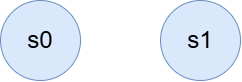
\includegraphics[width=4cm]{./img/ex-stratego-prog-d-1.png}
\subcaption{Dependence graph for \texttt{Null}.}
\label{fig:ex-stratego-program-d-graphs-1}
\end{subfigure}%
\begin{subfigure}{0.33\textwidth}
\centering
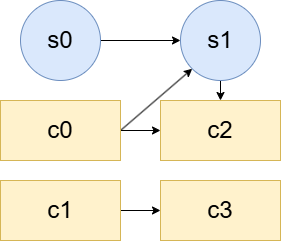
\includegraphics[width=4cm]{./img/ex-stratego-prog-d-3.png}
\subcaption{Dependence graph for \texttt{A}.}
\label{fig:ex-stratego-program-d-graphs-2}
\end{subfigure}%
\begin{subfigure}{0.33\textwidth}
\centering
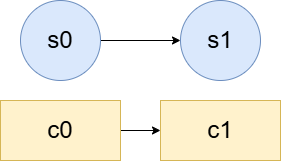
\includegraphics[width=4cm]{./img/ex-stratego-prog-d-2.png}
\subcaption{Dependence graph for \texttt{B}.}
\label{fig:ex-stratego-program-d-graphs-3}
\end{subfigure}

\caption{Dependence graphs of the example Stratego program in \autoref{fig:ex-stratego-program}.}
\label{fig:ex-stratego-program-d-graphs}
\end{figure}

\section{Finding Fusion Opportunities}
\label{sec:finding-fusion-opportunities}
For every call node in the dependence graph, the algorithm checks whether it can be merged with another call. It does this by merging their nodes in the graph. If this does not cause a cycle, the fusion is legal. Edges between the nodes being merged are simply removed and do not cause a self-loop.

As an aside, ignoring self-loops created in this manner makes it legal to fuse two call nodes that have a dependency relation without explicitly preserving their relative ordering. The reason this is legal is because their relative ordering must be preserved through dependency edges between statement nodes\footnote{We refer to the TreeFuser paper for a formal proof of the soundness of fusion\cite{SakkaS017}}. Of course, the relative ordering to all other nodes is always preserved when fusing.

We can only attempt to fuse calls that descend into the same child. For example, it is not legal to fuse a call that goes into the left child of a binary tree from one traversal with a call that descends into the right child from another traversal. Fusion can also only happen across different traversals, so the algorithm never attempts to fuse two calls that originate from the same traversal function.

Note that a single program may have multiple opportunities for fusion. Some fusions may exclude other opportunities, while some may be able to be combined. The algorithm attempts to exhaustively explore every possible combination of fusions, but this may quickly become prohibitively expensive for larger programs. 

Returning to the example dependence graphs shown in \autoref{fig:ex-stratego-program-d-graphs}, fusion proceeds as follows. The graph for \texttt{Null} does not contain any calls and as such there are no fusion opportunities. The graph for \texttt{B} has two calls that are from different traversals and traverse down into the same child. The algorithm attempts to fuse them. This results in the graph shown in \autoref{fig:ex-stratego-program-d-graphs-fused-1}, which does not contain a cycle. This means that the fusion is legal.

The graph for \texttt{A} contains four calls. There are two fusion opportunities: \texttt{c0} with \texttt{c2}, and \texttt{c1} with \texttt{c3}. The latter is a legal fusion and the resulting graph is shown in \autoref{fig:ex-stratego-program-d-graphs-fused-2}. 

The algorithm will also attempt to fuse \texttt{c0} and \texttt{c2}. However, this results in the graph shown in \autoref{fig:ex-stratego-program-d-graphs-fused-3}, which contains a dependency cycle. That means that this particular fusion is not legal.

\begin{figure}
\begin{subfigure}{0.33\textwidth}
\centering
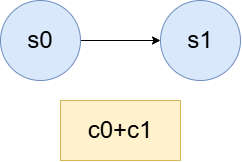
\includegraphics[width=4cm]{./img/ex-stratego-prog-d-2-fuse.png}
\subcaption{Fused graph for \texttt{B}.}
\label{fig:ex-stratego-program-d-graphs-fused-1}
\end{subfigure}%
\begin{subfigure}{0.33\textwidth}
\centering
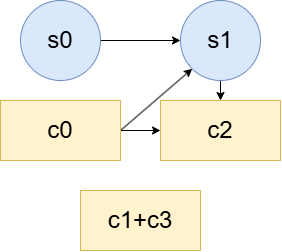
\includegraphics[width=4cm]{./img/ex-stratego-prog-d-3-fuse.png}
\subcaption{Fused graph for \texttt{A}.}
\label{fig:ex-stratego-program-d-graphs-fused-2}
\end{subfigure}%
\begin{subfigure}{0.33\textwidth}
\centering
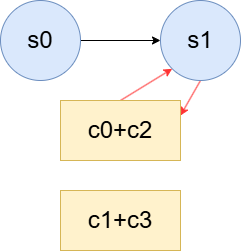
\includegraphics[width=4cm]{./img/ex-stratego-prog-d-3-fuse-illegal.png}
\subcaption{Illegal fused graph for \texttt{A}.}
\label{fig:ex-stratego-program-d-graphs-fused-3}
\end{subfigure}

\caption{Fused dependence graphs of the example Stratego program in \autoref{fig:ex-stratego-program} and \autoref{fig:ex-stratego-program-d-graphs}.}
\label{fig:ex-stratego-program-d-graphs-fused}
\end{figure}

\section{Fused Traversal Synthesis}
If the dependency analysis predicts one or multiple fusions, this will be evident from the fused nodes appearing in the dependence graph(s). However, these graphs need to be turned back into code that can execute the fused traversal.

The first step is to determine a new execution order. For every dependence graph, the algorithm places all the nodes in topological order based on the dependency edges present. This is always possible because the graph is guaranteed to be acyclic. Each graph may have a different number of nodes and a different resulting topological order.

As an aside, note that information about the original program order is ignored. This means that, even if the algorithm was not able to perform any fusion, the synthesized program may produce a different execution order. For example, it may be legal to change a top-down traversal to a bottom-up traversal in some cases. This is a feature of the algorithm, and it may be possible to use heuristics to prefer certain execution orders over others. In the prototype algorithm, we simply pick an arbitrary topological order without preference.

From the fused example graphs in \autoref{fig:ex-stratego-program-d-graphs-fused}, we get the following topological orders:
\begin{lstlisting}[style = mystyle_fused_stratego]
    Null : s0 -> s1
    A : s0 -> c0 -> c1+c3 -> s1 -> c2
    B : s0 -> c0+c1 -> s1
\end{lstlisting}

The algorithm first generates a \texttt{main} function that performs a match\footnote{\label{note-match-cong}Refer to \autoref{sec:additional-stratego-syntax} for an explanation of matches and congruences} on the current constructor, and calls a \texttt{main} function specialized to that constructor. For this example, it looks like this:
\begin{lstlisting}[style = mystyle_fused_stratego]
    f_main = ?A(_, _, _, _) < f_main_A + ?B(_, _) < f_main_B + ?Null() < f_main_Null + id
\end{lstlisting}

The algorithm then generates these \texttt{main} functions for every constructor, in which all statements from that constructor's topological order are inserted in order. Rewrite rule statements are inserted as invocations of the rule. Calls are inserted as a match on the constructor, with a function call then invoked on the correct child. The function we call also needs to be generated. To do this, we need the child and traversal annotations present on these nodes.

For example, when looking at the topological order for the \texttt{A} constructor in this example, the call \texttt{c0} is a call on the first child, originating from the first traversal. \texttt{c1 + c3} is a call on the second child, originating from both the first and second traversals (that is, from all traversals). Then, these statements together will be translated into the following Stratego code\footnote{See \ref{note-match-cong}}:
\begin{lstlisting}[style = mystyle_fused_stratego]
    A(f_0, f_main, id, id)
\end{lstlisting}

\texttt{f$\_$main} already exists and will select the correct \texttt{main} function for the constructor that the child happens to be. \texttt{f$\_$0} will have to be generated. It will also be a selector function that performs matches on the constructor, to then invoke the correct \texttt{f$\_$0} for the constructor in question. It looks like this:

\begin{lstlisting}[style = mystyle_fused_stratego]
    f_0 = ?A(_, _, _, _) < f_0_A + ?B(_, _) < f_0_B + ?Null() < f_0_Null + id
\end{lstlisting}

Generating these type-specialized functions is similar to generating the type-specified \texttt{f$\_$main} functions. The difference is that now only statements that originate from one of the selected traversals are inserted. For \texttt{f$\_$0}, that means we ignore all statements that do not originate from the first traversal. For \texttt{A}, that means \texttt{s1} and \texttt{c2} are ignored. \texttt{c1+c3} is inserted because it originates from both the first and second traversal. However, its part originating from the second traversal \textit{is} ignored. Whereas normally this call would generate a call to \texttt{f$\_$main}, it now also generates a call to \texttt{f$\_$0}. Then, we have

\begin{lstlisting}[style = mystyle_fused_stratego]
    f_0_A = r1; A(f_0, f_0, id, id)
\end{lstlisting}

The full synthesized code for this example is displayed in \autoref{fig:ex-stratego-program-fused-code}.

\begin{figure}
\begin{lstlisting}[style = mystyle_fused_stratego]
f_main = ?A(_, _, _, _) < f_main_A + ?B(_, _) < f_main_B + ?Null() < f_main_Null + id
f_0 = ?A(_, _, _, _) < f_0_A + ?B(_, _) < f_0_B + ?Null() < f_0_Null + id
f_1 = ?A(_, _, _, _) < f_1_A + ?B(_, _) < f_1_B + ?Null() < f_1_Null + id

f_main_A = r1; A(f_0, f_main, id, id); r2; A(f_1, id, id, id)
f_main_B = r1; B(f_main, id); r2
f_main_Null = r1; r2

f_1_A = A(id, f_1, id, id); r2; A(f_1, id, id, id)
f_1_B = B(f_1, id); r2
f_1_Null = r2

f_0_A = r1; A(f_0, f_0, id, id)
f_0_B = r1; B(f_0, id)
f_0_Null = r1
\end{lstlisting}

\caption{Synthesized fused code for the example Stratego program of \autoref{fig:ex-stratego-program}.}
\label{fig:ex-stratego-program-fused-code}
\end{figure}


\section{Limitations}
\label{sec:limitations}
In this section, we will discuss the limitations of our algorithm and the POC implementation in more detail.

First, and most importantly, we note that the algorithm cannot find all possible fusion opportunities. This is an inherent limitation of the algorithm: checking whether a fusion is legal using dependency analysis is sound but incomplete. In other words, if a fusion is illegal, there must be a dependency violation, but if there is a dependency violation, a fusion is not necessarily illegal. This means that the algorithm will never fuse something illegally, but it may not fuse all programs that can be fused. A more sophisticated dependency analysis could theoretically find more possibilities, but it cannot avoid the fact that a dependency violation does not always imply a fusion is illegal.

In contrast, there are a few limitations that exist only in the POC implementation of the algorithm. This does not necessarily imply they are easy to implement, but it is certainly possible to do so in theory. These are, in no particular order: constraints on constructor types (e.g. lack of list types), lack of support for side effects, constraints on the structure of the input program, required type declarations, and the lack of support for conditional traversals. We will discuss for each of these limitations in short how it might be addressed.

The constraints on constructor types are relatively straightforward to address. It is simply a matter of information extraction from the source program. Of course, the dependency analysis will also have to be updated to support list types, but it would not require any fundamental changes to the algorithm.

The lack of support for side effects is more complex. Of course, the algorithm would have to be able to correctly identify side effects. If those can be extracted from the source program, there would also have to be some more thorough changes to the dependency analysis algorithm. Side effects may have to be analyzed as reads and writes to global locations.

The constraints on the structure of the input program come down mostly to a matter of information extraction. However, it is important to remember that allowing for more complex input programs may also complicate code synthesis after fusion. It is important that no critical information about the structure of the program is lost, so that the program can be correctly synthesized back together in the end.

The required type declarations are an interesting limitation. It may be possible in theory to infer types for all constructors, removing the need for an explicit declaration. However, if this inference is less strict, some fusion opportunities may be lost.

Finally, the lack of support for conditional traversals is mostly a matter of code synthesis. Conditional traversals can be simulated with unconditional calls that immediately return\cite{SakkaSN019}. Again, it is important to keep in mind that there needs to be support for this in terms of information extraction (and retention throughout dependency analysis). However, if this can be done, the challenge is mostly a matter of synthesizing a correct program.